\usetikzlibrary{decorations.pathreplacing}
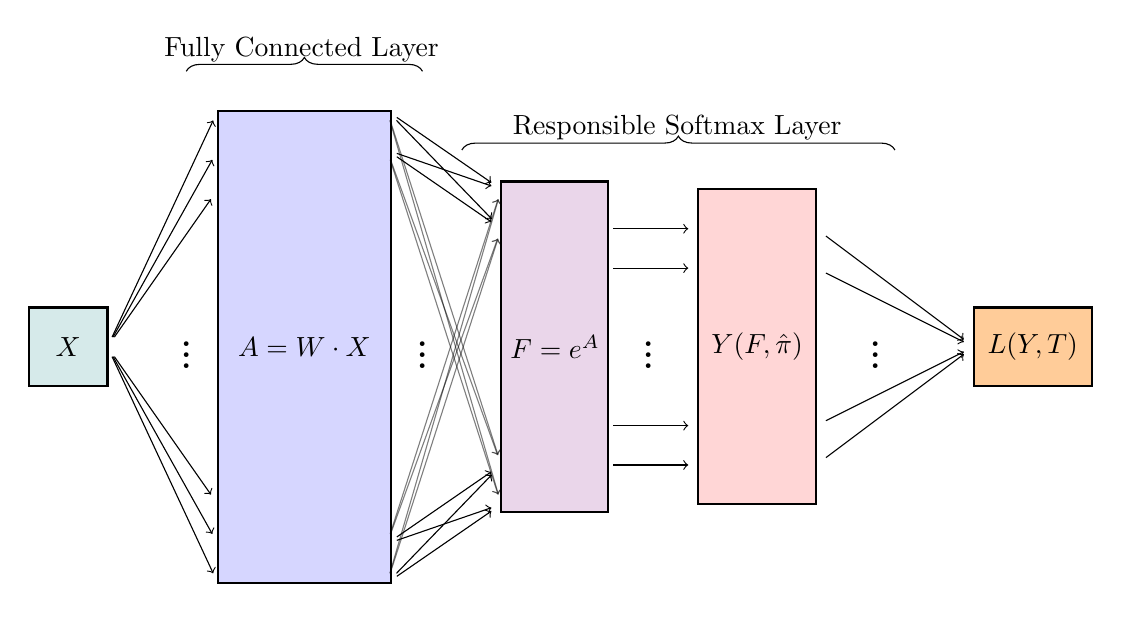
\begin{tikzpicture}
% Layer boxes and labels
\draw  [fill = teal!20, fill opacity = .8, thick ](-7.5,0) rectangle (-6.5,-1);
\node at (-7,-0.5) {$\bm X$};
\draw  [fill = blue!20, fill opacity = .8, thick ](-5.1,2.5) rectangle (-2.9,-3.5);
\node at (-4,-0.5) {\(\bm A =\bm W\cdot \bm X\)};
\draw  [fill = violet!20, fill opacity = .8, thick ](-1.5,1.6) rectangle (-0.14,-2.6);
\node at (-.815,-0.5) {$\bm F = e^{\bm A}$};
\draw  [fill = red!20, fill opacity = .8, thick ](1,1.5) rectangle (2.5,-2.5);
\node at (1.75,-0.5) {$\bm Y(\bm F,\hat{\bm\pi})$};
\draw  [fill = orange!50, fill opacity = .8, thick ](4.5,0) rectangle (6,-1);
\node at (5.25,-0.5) {$L(\bm Y,\bm T)$};
% Connections between first and second layer
\node (v1) at (-6.5,-0.5) {};
\node (v2) at (-5.1,2.5) {};
\node (v3) at (-5.1,2) {};
\node (v4) at (-5.1,1.5) {};
\node at (-5.5,-0.5) {\huge{$\vdots$}};
\node (v6) at (-5.1,-3) {};
\node (v7) at (-5.1,-3.5) {};
\node (v5) at (-5.1,-2.5) {};
\draw [->] (v1) edge (v2);
\draw [->] (v1) edge (v3);
\draw [->] (v1) edge (v4);
\draw [->] (v1) edge (v5);
\draw [->] (v1) edge (v6);
\draw [->] (v1) edge (v7);
% Connections between second & 3rd layer
\node (v8) at (-2.95,2.5) {};
\node (v11) at (-2.95,2) {};
\node (v15) at (-2.95,-3) {};
\node (v12) at (-2.95,-3.5) {};
\node (v9) at (-1.5,1.5) {};
\node (v10) at (-1.5,1) {};
\node (v14) at (-1.5,-2) {};
\node (v13) at (-1.5,-2.5) {};
\draw [->] (v8) edge (v9);
\draw [->] (v8) edge (v10);
\draw [->] (v11) edge (v9);
\draw [->] (v11) edge (v10);
\draw [->] (v12) edge (v13);
\draw [->] (v12) edge (v14);
\draw [->] (v15) edge (v13);
\draw [->] (v15) edge (v14);
\draw [->,opacity = .5] (v8) edge (v14);
\draw [->,opacity = .5] (v8) edge (v13);
\draw [->,opacity = .5] (v11) edge (v14);
\draw [->,opacity = .5] (v11) edge (v13);
\draw [->,opacity = .5] (v15) edge (v9);
\draw [->,opacity = .5] (v15) edge (v10);
\draw [->,opacity = .5] (v12) edge (v9);
\draw [->,opacity = .5] (v12) edge (v10);
\node at (-2.5,-0.5) {\huge{$\vdots$}};
% Connections between 3rd and 4th layer
\node (v16) at (-0.2,1) {};
\node (v18) at (-0.2,0.5) {};
\node (v20) at (-0.2,-1.5) {};
\node (v22) at (-0.2,-2) {};
\node (v23) at (1,-2) {};
\node (v21) at (1,-1.5) {};
\node (v19) at (1,0.5) {};
\node (v17) at (1,1) {};
\draw [->] (v16) edge (v17);
\draw [->] (v18) edge (v19);
\draw [->] (v20) edge (v21);
\draw [->] (v22) edge (v23);
\node at (0.375,-0.5) {\huge{$\vdots$}};
% Connections between 4th and 5th layer
\node (v25) at (4.5,-0.5) {};
\node (v24) at (2.5,1) {};
\node (v26) at (2.5,0.5) {};
\node (v27) at (2.5,-1.5) {};
\node (v28) at (2.5,-2) {};
\draw [->] (v24) edge (v25);
\draw [->] (v26) edge (v25);
\draw [->] (v27) edge (v25);
\draw [->] (v28) edge (v25);
\node at (3.25,-0.5) {\huge{$\vdots$}};
% Layer labels
\draw [decorate,  decoration={brace,  amplitude=5pt}] (-5.5,3)--(-2.5,3) node[above, xshift =-43.7]{Fully Connected Layer};
\draw [decorate,  decoration={brace,  amplitude=5pt}] (-2,2)--(3.5,2) node[above, xshift =-78.7]{Responsible Softmax Layer};
\end{tikzpicture}